\documentclass[12pt,a4paper]{article}
\usepackage[utf8]{inputenc}
\usepackage[english]{babel}
\usepackage{amsmath}
\usepackage{amsfonts}
\usepackage{amssymb}
\usepackage[left=2.00cm, right=2.00cm]{geometry}
\usepackage{graphicx}
\usepackage{xcolor}
\usepackage{natbib}
\usepackage{comment}
\usepackage[most]{tcolorbox}
\newcommand{\Zu}[1]{\textcolor{blue}{\rm{Zu cmmt:} #1 \rm}}
%\usepackage[style=authoryear-icomp,sorting=anyt]{biblatex}

%\addbibresource{Biblio_deepbios.bib}
%\graphicspath{C:\Users\Rodrigo\Desktop\Papers_ON GOING\TREE_Modelling}

\begin{document}
\title{Sustainability discovery in eco-evolutionary diversification-inspired federated networks}%Title as in the FET EU proposal

\maketitle
\noindent \author{Rodrigo Riera$^{1,2,*}$, Ali Vadathi$^{3}$, Francisco Bald\'o$^{4}$, Gian Marco Palamara$^{5,6}$, Oskar Hagen$^{x}$, Pengjuan Zu$^{y}$, Victor M. Egu\'iluz$^{z}$, and Carlos J. Meli\'an$^{8,9}$}
            \\
    %Discuss with David Alonso${^6}$ and Joaqu\'in Hortal${^7}$ about authorship
    %Potential coauthors: %JON NORBERG -- PAULO GUIMARAES
            
            \vspace{0.25 in}
            
  \noindent  $^{1}$IU-ECOAQUA, Departamento Biolog\'ia, Universidad de Las Palmas de Gran Canaria, Canary Islands, Spain\\
  $^{2}$Departamento de Ecolog\'ia, Facultad de Ciencias, Universidad Cat\'olica de la Sant\'isima Concepci\'on, Concepci\'on, Chile\\
  $^{3}$, Department of XX, University of Zurich, Switzerland\\
  $^{4}$Instituto Español de Oceanografía (IEO), C.O. de Cádiz, Cádiz, Spain\\
  $^{5}$Department of Systems Analysis, Integrated Assessment and Modelling, Eawag Center for Ecology, Evolution and Biogeochemistry, Switzerland\\
  %$^{6}$Theoretical and Computational Ecology, Center for Advanced Studies of Blanes, Girona, Spain\\
  %$^{7}$Departamento de Biogeograf\'ia y Cambio Global, MNCN, Madrid, Spain\\
  $^{8}$Department of Fish Ecology and Evolution, Eawag, Centre of Ecology, Evolution and Biogeochemistry, Switzerland\\
  $^{9}$ Institute of Ecology and Evolution, Aquatic Ecology, University of Bern, Baltzerstrasse 6, CH-3012, Bern, Switzerland.\\
\vspace{0.25 in}

  $^{*}$corresponding author: rodrigo.riera@ulpgc.es

\newpage
\begin{abstract}
Identifying the coupling between biological organisms, human activity and the environment is critical to understand the fate of the Earth system. This effort mostly relies on the expertise coming from different disciplines emphasizing the need for objective assessment of direct and indirect interactions. Connecting large datasets combining natural ecosystems with human activities to infer causal links and novel sustainability paths in evolving  ecosystems remains at a very incipient stage.  Here we propose a unified computational framework that capitalize large datasets to infer connections between variables. Here, we connect data, causal and discovery knowledge graphs into a unified computational sustainability framework to explore gradients of model complexity coupling biological-human datasets for large ecosystems. Secondly, we validate our approach with a case study focusing on ocean sustainability in federated networks, where many heterogeneous groups of species, humans, and technologies coexist exploiting resources. Finally, we contrast Bayesian causal networks with and without eco-evolutionary diversification of traits and technologies to show how novel sustainability discovery paths can be achieved. We discuss our approach in the context of science-based technologies aiming at connecting knowledge-inspired societies to global sustainability challenges.

\end{abstract}



\begin{comment}
\Zu{In general, I feel there are many terms in abstract that are not easy to get their real meanings without giving proper explanations, and it is not very obvious to get the relations/connections of these terms. As commented in the text: what is 'biological-human interactions'; what is 'earth and environmental dynamics'; why one is fine-grained and the other is coarse-grained; what does this to do with 'Biodiversity science' here.\\
Perhaps the logic flow can be: 1) the complexity of ecosystems (incl. different layers/scales of ecosystem compositions (static), and different factors that influence ecosystem dynamic). 2) the importance and challenges in predicting (projecting to future) and understanding (mechanistically) ecosystem (as Fig. 3). 3) the key questions and innovation of the project: aim to figure out how knowledge (for prediction and understanding) changes along different gradients of complexity? A sustainable workflow/technique on how to process data --> knowledge --> applications (promote more sustainable ecosystems). This developed technique is sustainable because it is automated, and output can be updated when feeding new data (it evolves with data).)\\
This is what I understand about from reading the manuscript and the discussion today. Maybe there are some other points I have missed.}


The merging of pattern- and process-based methods and the building
of theory to merge knowledge and predictive power is not taken
place. Theories play a pivotal role in providing explanations to
what, at first, might seem to be a series of disconnected, even
paradoxical, patterns. We provide here a framework connecting
synthesis between pattern- and process-driven research. Our approach
integrates deep learning networks with process-based methods, i.e. deep
process-based learning network to infer patterns and processes
underlying large and integrated databases. We show a case study
using a deep process-based learning network to explore the strength of
coupling between layers and the dimensionality in Biodiversity and
Environmental databases. We validate our approach with a case study focusing on the sustainability of the ocean in federated networks, where many heterogeneous groups of species, humans, and technologies coexist exploiting resources in complex ecosystems. Merging process-based approaches and
data-driven deep learning networks might play a critical role in
deciphering the strength of the coupling between Earth and
biodiversity systems in rapidly changing landscapes. Lastly, this project not only sets out to deliver novel computational sustainability approaches but also provides fully reproducible open-source software solutions of a science-enabled technology to connect knowledge-inspired societies to global sustainability challenges.
\end{comment}

\newpage

\section{Introduction}

Human footprint is pervasive worldwide without untouched wilderness \citep{marconcini2020outlining, mcdowell2020pervasive}. Biodiversity research is a top priority to ensure ecosystem conservation and halting habitat loss and fragmentation \citep{brum2017global}. Unraveling the linkages among physico-chemical processes, environmental drivers, internal regulatory processes at the population, community, and ecosystem levels; and the role of human intervention is essential for effective management and sustainability \citep{hobbs2011intervention}. Recent approaches have shown that these interactions can result in complex dynamical behavior including sudden shifts in ecosystem states and extinction patterns of populations and communities \citep{newman2019scaling}. Biodiversity science has expanded in a wide range of sub-disciplines throughout the last decades \citep{loreau2010challenges}, yet, the integration of diverse databases to decipher the sustainability properties of exploited ecosystems is at a very incipient stage. Exploited ecosystems need to be addressed from a broad-scale and synthesis perspective, because of the complex scientific problems concerning the description and prediction of biodiversity patterns and processes using data from genes, individuals, communities, and ecosystems across temporal and spatial scales \citep{chase2018embracing}, as well as, their implications on current and future societal challenges such as climate change, human health, and poverty \citep{cardinale2012biodiversity, turner2012global}. In 2015, 17 Sustainable Development Goals (SDGs) were set by the United Nations. These SDGs identify current global problems that are shared across the globe and require an immediate solution.  The  implementation  of  SDGs requires a local-to-global framework that would provide a global yet local plan of action. Computational thinking can  contribute  to providing a universal framework and collective structure for problem-solving through processes that are suitable at a local-scale for each population. The applicability of computational approaches as a real-world environmental problem-solving tool is in an incipient stage \citep{rabiee2017abstraction}. Further research is needed to develop modelling approaches providing environmental-sustainable solutions for global-shared and local-specific systems.

Connecting exploited to biodiversity maintenance is calling for technologies to discover novel ways of sustainable exploitation. Novel technologies for data integration from different fields, {\it i.e.}, environmental, social, biodiversity and Earth science data, can uncover new patterns, causal relationships and new paths to reach sustainable exploitation while maintaining biodiversity. This is of paramount importance since the patterns observed in the collapse of ecosystems are usually driven by the interactions among different agents, sectors, and spatio-temporal scales. Major technological advances in computing power, remote sensing, and omics, i.e. genomics, transcriptomics, proteomics, metabolomics, among others, have provided new tools to improve understanding of biodiversity patterns \citep{craven2019evolution}. Bayesian networks are promising tools to fill this gap since developing causality-targeting modelling approaches.
These advances within the framework of knowledge-based societies place great expectations on data-driven intelligent machines to face global sustainability challenges. In this regard, database integration to facilitate the discovery of sustainable paths in resource exploitation, the major feature of computational sustainability, is a major issue revolving around data-driven intelligent machines and knowledge-based societies \citep{Gomesetal2019}. However, there are still considerable limitations regarding the integration of data and modelling approaches, especially those concerning the (i) connections between oversimplified simple models and more realistic counterparts, and (ii) computational constraints when developing complex and realistic models. There have recently been fast improvements in methods delivering explainable and complex models integrating heterogeneous data, and also, these models challenge the limits to computational speed to deliver robust conclusions \citep{rodrigues2014integrative}. Moreover, there is still a long way to go through interdisciplinary fields that promote synergies among societal, economic, and environmental resources within the framework of sustainability. The main core sustainability themes remain dispersed and integrated only superficially: (i) Biodiversity and Conservation; (ii) Balancing environmental and socio-economic needs; and (iii) Energy and renewable resources. Only recently, new tools for data integration and analysis can facilitate the integration required to gain an understanding between exploited and sustainable ecosystems for species-rich and human-dominated ecosystems.

Here we aim to explore model complexity gradients using Bayesian networks, causality graphs, and novel paths to uncover relations among the data, and to broaden computational sustainability concepts (see Table and methods). Our approach has the potential to integrate process- and pattern-based models from simple to more complex ones to optimize a wide range of resources, {\it i.e.}, diverse prey communities, environmental factors, fishing and the technologies used to exploit resources and the economic or societal impacts. Scaling up from micro-ecological processes requires the use of data-driven evidence. Finally, it is essential that data from implementation monitoring are linked to decision-making through data integration and model complexity gradients robustly explored. 

Therefore, integrating data, causality and novel paths to connect exploitation and sustainability criteria in complex ecosystems can assist both policy makers and researchers to determine the most useful type of research at different stages of scaling up processes. This process is of paramount importance to avoid failure of initiatives to influence the society, and the "know-do gap" - the gap between what is known in research and what gets implemented \citep{catford2009advancing}. The integration of models ranging from simple models to deep learning complex models will expand the reach of an intervention to new settings or target groups and is accompanied by a systematic strategy to achieve this objective \citep{milat2014increasing}. Yet, scarce studies deal with frameworks, approaches and methods for effective scale-up interventions \citep{wigboldus2013towards, yamey2012barriers}. The integration of deep learning networks with process-based methods providing evidence-to-practice frameworks is pivotal for policy makers, practitioners and stakeholders to scale up global interventions. Computational sustainability is an interdisciplinary discipline that needs to be built from a federated network, potentially more powerful than centralized ones. Many computational sustainability problems require making decisions through time. Solving these problems involves maximizing the expected reward by finding the most suitable that can generate future hypotheses without considering the simulator to run. Another approach consists of the recently developed "stochastic computers" \citep{borders2019integer}, energetically more efficient than conventional ones, and perform faster and more complex calculations. Yet, complex and integrative computational analyses are laborious and extremely time-consuming \citep{rodrigues2014integrative}, especially those related to big data involved in deep learning approaches. Several alternatives have been recently developed such as the development of off-policy evaluation using the Model Free Monte Carlo (MFMC) method \citep{fonteneau2010model}. 

Bayesian networks provide a way to calculate the joint probability distribution of variables succinctly and computationally feasible \citep{pearl2011bayesian}. Conditional probabilities of Bayesian networks are pivotal to calculate fitting data. A subset of Bayesian networks is Causal Bayesian networks (CBNs), where the relationship between variables is causal. There are algorithms to automatically discover a class of causal relationships between variables that best match the data. Combining automatic causal discovery algorithms and expert knowledge, we can find relationships among variables that are new and informative. Bayesian networks have been explored maintaining the same number of nodes and links. However, nodes are changing entities that can predict better estimations to the empirical patterns. Diversification of biological systems offers here an unexplored avenue for inspiration of new computational approaches. However, diversifying ecosystems are not used for sustainability discovery yet, despite the rapid changes of traits and interactions observed in overexploited, experimental and theoretical systems \citep{Hairston2005, Walsh2006, Fussmann2007, Trugman8532}. Biological systems are characterized by feedbacks between the ecology and evolution of interacting traits, the eco-evolutionary feedbacks, to produce novel traits with new functionalities \citep{Govaertetal2019}. This results in new computational properties, like new cooperation and competition strategies and information processing capabilities. Diversification usually occurs in heterogeneous ecosystems with limited resources where many distinct groups need to develop specialized traits and strategies to obtain resources. The outcome is the formation of consortia and more broadly federated networks composed of phylogenetically and ecologically distinct groups. Conventional Artificial Intelligence (AI) is rapidly moving towards explainable and discovery pattern inference \citep{Iten2020a} but often avoids evolutionary diversification for exploring new computing capabilities \citep{Real2020}. The same situation occurs for artificial neural networks that also make limited use of novel computing capabilities as a consequence of new interactions and traits \citep{Schmidhuber:2015}.


\begin{comment}
The goal of this project is to implement eco-evolutionary diversification-inspired solutions to perform computational sustainability discovery based on rapidly diversifying traits and interactions. The exploitation of emerging interactions, strategies and traits will allow us to create novel discovery solutions for natural ecosystems facing sustainability challenges like overexploitation of the ocean, where harvesting renewable resources are beyond the diminishing returns for many species and ecosystem resources \citep{Paulyetal1998, Mastrangelo2019}. Why should we go deeper into diversifying networks for computational sustainability? With connections and traits represented in a spatially distributed network, as found in natural ecosystems, diversification is an avenue to harvest renewable resources because most innovations in ecosystems are connected to new sensing and information processing cues to detect and exploit resources. This allows considering not only evolutionary processes changing traits and agents (i.e., plasticity and other sources of variation), but the formation of new entities to quantify new scenarios for sustainability that substantially deviate from evolutionary computation considering only changes and not diversification processes. This also allows representing real-time solutions for ever-changing renewable resources, which is a key problem in many digital and natural systems. We here show a case study using a deep process-based learning network to explore the strength of coupling between layers and the dimensionality in Biodiversity and Environmental databases. We test this approach with a case study focusing on ocean sustainability in federated networks, where species, humans, and technologies coexist exploiting resources in complex and rapidly changing seascapes. To show the capabilities of the approach, we will address full reproducibility, automation, visualization, and reporting (Figure 1). Data integration, causality and diversity may provide a new technology to improve ecosystem sustainability relevant to community-rich digital and natural ecosystems.

%\begin{tabular}%[leftmargin=2cm]

\begin{enumerate}%[\hspace{-0.0 in}(G1)]
%\setlength\itemsep{-0.3em}
   % \vspace{-0.15 in}
    \item To extend existing theories of eco-evolutionary diversification and AI-inspired solutions to decipher the factors driving sustainability discovery in federated networks. This will allow us to identify novel solutions for ecosystem sustainability.
% \vspace{-0.15 in}
    \item To investigate how spatio-temporal evolutionary diversification and AI-inspired networks mimic the empirical patterns of natural and socio-technological ecosystems when heterogeneous human groups, technologies, and species coexist.
% \vspace{-0.15 in}    
    \item To develop fast, reproducible and automated eco-evolutionary diversification-inspired sustainability discovery prototypes for real-time information processing tasks.
% \vspace{-0.15 in}    
    \item To obtain principles of sustainability discovery for prediction in federated networks when diversification in interactions and traits occurs in a large and heterogeneous set of species, technologies and human groups. 
\end{enumerate}

\end{comment}

Taking into account many changing factors to understand complex and large datasets (Figure 1 and Table X) present many challenges. First, biodiversity data is typically scarce and biased (\citep{hortal2015seven}). Although an increasing number of ecological datasets are available, most, if not all, of them are of uneven coverage and quality (Table 1). Second, many patterns have emerged with conflicting explanations usually depending on the spatial and temporal scales of the observations (see Figure 1 and Table 2). Lastly, progress in biodiversity sustainability relies on unifying different theories and datasets in order to explain as many natural patterns with as few principles as possible. Also, merging methods from distinct disciplines can increase our predictive understanding power to develop and test new theory (\citep{reichstein2019deep}). Here we take on a composite of approaches to fully integrate empirical data and theory, particularly through guiding the attention of researchers onto integrating datasets to account for several biological levels and spatio-temporal scales \citep{melian2018deciphering}, \citep{poisot2019data}.

%Make better flow between computational sustainability and data, causal, and discovery knowledge graphs -- make clear the case study (fish data from North Sea, state clear!!!)
Recent approaches in ecology and evolution have introduced deep learning methods for labelled data, from which selection modes and demographic history can be jointly inferred \citep{sheehan2016deep}. The fusion of models coming from AI and theory in biodiversity research would shed light on process-based scenarios of biodiversity sustainability for large datasets. Yet, most approaches applying deep learning or network methods in biodiversity have mostly focused on one level of biological organization, {\it e.g.}, genes, species or communities, without considering the interaction among them nor the interactions with technological traits and human-disturbances on ecosystems. Also, these studies are single-focused and limited to taxonomic diversity, with no consideration of other emerging diversity dimensions \citep{weiss2019unifying}. Biological systems are composed of many layers (Figure 1), and they can contain interdependent hierarchies and feedbacks with interacting learning entities within and between layers. The number of layers needed for predicting and understanding biological patterns still remains overlooked. This is specifically complex in the Anthropocene, with the widespread role of human-driven disturbances. Bayesian network models connected to deep process-based models accounting for several layers and interactions within and between the layers are going to be important to maintain sustainable ecosystems in the long-term \citep{fontaine2011ecological}, \citep{melian2018deciphering}, \citep{reichstein2019deep}). Data science and biological systems share pivotal properties, but their full potential has not been sufficiently explored \citep{schmidhuber2015deep}. Therefore, exploring deep learning network topologies accounting for feedbacks within and between layers is a first step towards understanding biodiversity dynamics using deep process-based learning networks.

\section{Methods}




\subsection{Bayesian networks}
Sustainable ecosystems are complex ones that incorporate several parameters and heterogeneity across levels. Deciding which level of complexity best captures real ecosystems for understanding sustainability is a major challenge today. Modeling such systems requires tools such as agent-based models integrating data from many fields. ABMs can show emergent properties and many of the features of a system that are often absent in analytical models. A drawback of ABMs is that they are computationally expensive. Therefore, methods making a continuum from analytical models to ABMs are required to quantitatively evaluate the pros and cons of both approaches. Analyzing ABMs needs exploring a large parameter space, which is usually not feasible. A workaround for this limitation is building emulators, which are mathematical formulations (machine learning models) that can estimate the complex behavior of a simulation given different inputs. We can use either traditional machine learning algorithms or deep learning for this endeavour. Traditional ML algorithms have limited predictive power and may not be able to predict complex high-dimensional data. Deep learning is often the choice when there is a large number of training samples. But such a large number of samples are not easy to produce when a single simulation run takes long. A solution to this problem is to find an optimal deep learning architecture. This has been shown to replace complex simulations with very few input data (\cite{Kasim2020}). There are different optimization methods for finding the best architecture (\cite{Elsken2018}). Here, we explore architectures with different degrees of complexity aiming to unify analytical to ABMs scenarios to understand the paths to sustainable ecosystems. 

%EMERGING HETEROGENEOUS DATA, different sources, time series, geographic areas. Federated networks will be used to integrate all data regardless their nature/heterogeneity, etc.

Emulators are required when our available data is incomplete. This may occur in two scenarios, (i) When we are producing simulated data and those simulations are too time-consuming to explore all parameter combinations; (ii) When we have experimental data that are hard to gather and do not cover all possible parameter combinations. Emulators can predict how the system (computational or real) would behave with new parameter values. These predictions would then be valuable to create knowledge graphs to answer sustainability questions (i.e., finding discovery paths that improve sustainability in the exploitation of the ecosystem).

Probability graph models (PGMs), a subset of which are Bayesian Networks (BNs), are a powerful tool for mixing available data (from computer simulations, experiments, and expert knowledge) to gain a comprehensive understanding of a complex ecosystem. An advantage of BNs is that they provide probabilistic answers taking into account the uncertainties in data collection and outputs. In BNs are directed acyclic graphs (DAG) that show causation between parameters. They allow us to explore the effect of changing one parameter on parameters that are connected to it directly and indirectly.

%Sampling network: selection bias, missing data, latent variables
%For example 

%initial filter and constraints (node and link removal)
%Search space
%Fitting

%%%%%%%%%%%%%%%%%%%%%%%
\subsubsection{Diversifying traits and technologies}
Why do we need to explore two scenarios, one without trait and technology change and the other with changes? How do these two scenarios relate to the main questions to be addressed? 

We explore Bayesian networks in two different scenarios: One scenario without trait and technology changes and a second done with trait and technology changes. 

We infer the graphs in the two scenarios to provide the direct and the indirect interactions underlying causal and novel relationships .... to sustainability paths

Interpretation of the results with and without trait changes ...\\
The outcome of the analysis provides the weights $W_{ij}$ between pairs of nodes in the graph. The interpretation of the weights is the importance of variable $i$ in variable $j$. one possible goal is to extract connections in the marine food web. That is, fishing species $A$ affects positively or negatively species $B$. This food web can be compared with existing marine food webs and assess the performance of the approach, for example, the number of trophic interactions that we are able to capture. (A critique: do we need fishing activity to extract food webs? Probably we can come with a improve goal involving human activity.) 



\subsubsection{Exploring complexity gradients}

Protocol followed to explore dimensionality in the two scenarios. 


\subsection{Data, causal and discovery knowledge graphs}

\subsubsection{Data knowledge graphs}
\Zu{Following are added based on discussion with Carlos on 2nd March}\\
%"Computational sustainability aims to identify, formalize, and provide solutions to computational problems concerning the balancing of environmental, economic, and societal needs for a sustainable future". Gomes et al 2019
% I feel our computational sustainability is different from it(?)
In general, we can generate knowledge graphs at three different levels: (1) data knowledge graph (what we see), where we gain knowledge by summarising/categorising what we have observed. It is more descriptive and phenomenological. (2) Causal knowledge graphs (why we see what we see), where we aim to uncover the underneath mechanisms and explain what we observed in data knowledge graphs. (3) Discovery knowledge graph (what we haven't seen), where we try to discover novel knowledge from un-observed data (e.g. by employing theoretical reasoning and/or simulations).

\Zu{Here we could also add a few examples to explain what we mean for each level. One potential example is Darwin's hawkmoth where based on data knowledge graph (flower with long spur pollinated by long-tongue insect, short spur with short-tongue insect), and causal knowledge graph (nectar in flower spur as a reward for pollinator. a co-evolution case of spur length and insect tongue size), Darwin predicted (can we call it discover knowledge graph?) a super long-tongue insect as pollinator (later known as Xanthopan moth, be discovered 20 years after the prediction) when he only saw an orchid specimen with super long spur. Can also add other examples in different context (phenotype \& genetic control; maybe also one involve social-ecological effects as in our fishery case study}

\subsubsection{Causal knowledge graphs}

Most studies of data discovery focus on advanced analytics functions to gain insights, almost completely ignoring the heterogeneity of data sources \citep{azeroual2019solving}. Currently, only a few databases are semantically annotated from many data sources, e.g. gene ontology database (\citep{gene2021gene}), COVID-19 (e.g. https://www.who.int/emergencies/diseases/novel-coronavirus-2019/global-research-on-novel-coronavirus-2019-nco), among others. Ontology development is time-consuming and requires expert knowledge. It is also paired with data-driven research that checks the soundness of the ontology as it simultaneously seeks discovery. Unfortunately, software tools for mapping and linking different ontologies accounting for many data sources are at a very incipient stage of development \cite{nsf,KGcovid19,Oavida}. Evolutionary-based functions are of utmost importance to find datatype properties from ontologies and raw-data from biodiversity databases. Computational science is pivotal to explore algorithms to gain an understanding of the replicability of data heterogeneity contrasting different evolutionary algorithms. We here use computational approaches to explore the sustainability of the ocean database started in 1965 and currently containing 9 million entries, 1,612 species (i.e., 50 variables and traits per species), around 20 countries and 11 sampling methods (ref of database) (Figure 2).
\\
\begin{itemize}
    \item backwards to the causality literature in networks
    \item which algorithms have been used? How about evolutionary algorithms? and Evolutionary diversification algorithms?
\end{itemize}

Causal discovery from observable data has been extensively studied \citep{Rackauckas2020}. Many of these studies have used symbolic reconstruction of equations by symbolic regressions or evolutionary methods \citep{Koza1992, quade2016prediction, tanevski2020combinatorial}. A common gap in the literature is one where parameters represent eco-evolutionary diversification processes, and thus, discovery can be explored broadly. The classical view on biology-inspired information processing technologies is to consider plasticity without structural changes, or without diversification among many interacting components \citep{DARWISH2018231}. Recent experimental evolution studies show that rapid trait changes with new information processing capabilities are far more complex because adaptation and speciation occur even in sympatry forming new species and phenotypes \citep{Seehausen2014}. For example, eco-evolutionary dynamics strongly affect feedbacks between ecological and evolutionary processes, which influences trait changes to open new structural changes with new information capabilities \citep{Govaertetal2019}. Furthermore, recent studies suggest that the interplay between trait dimensionality, the covariance structure among traits, and adaptation is key to understand the emergence of new traits and information processing abilities to form novel computational sustainability discovery strategies in ecosystems \cite{zora172044}.\\

%So much novelty here -- lets see how far we go 
Eco-evolutionary diversification algorithms will be extended to deep process-based learning networks including traits and interactions driven by evolutionary changes to understand patterns in these systems. The search for causal knowledge discovery will be applied to the data knowledge discovery generated for the sustainability of the ocean, the largest realm on Earth and key actor of climate change affecting biogeochemical and physical processes. 

\subsubsection{Discovery knowledge graphs}
\\
\begin{itemize}
    \item cite refs showing the ideal of discovery
    \item is our discovery different from the classical drug discovery? If so, why?
\end{itemize}

Technologies in digital ecosystems around federated networks are rapidly increasing and mostly focus on decentralization, scalability and security fronts \cite{Androulaki2018,OceanProtocolFoundation2018,BigchainDBGmbH2018}. Yet, the implementation of eco-evolutionary diversification algorithms and their application to forecasting in global sustainability problems is still lacking. Recent studies have shown the importance of evolutionary search of mathematical and symbolic operations as building blocks to discover ML algorithms \citep{Real2020,Guimera2020}. Eco evolutionary diversification algorithms will help to decipher how interactions among heterogeneous groups evolve and learn to solve complex sustainability problems. Evolutionary dynamics explore open-ended languages of models with varying trait evolution functions to discover biologically inspired solutions in multidimensional systems \citep{Real2020} accounting for heterogeneous agents to discover novel biology-inspired solutions for the sustainability of the ocean federated network. Our understanding of the outcomes from diversified information processing systems formed by highly heterogeneous groups, a kind of large-scale meta-learning in the federated setting \citep{Dilley2016}, is currently quite limited. Therefore, new science-enabled approaches accounting for diversifying information processing in heterogeneous and highly dimensional systems are required. This allows the development of science-enabled technologies where heterogeneous agents with different interests find (non-optimal) solutions for the sustainable exploitation of ecosystems. Federated objects can be seen as ``neural networks'' containing many types of heterogeneous nodes with varying degrees of learning, connectivity and firing probabilities \citep{Maass2014,Maass2015}.


\subsection{Case study: Sustainability of the Ocean}

Heterogeneous biodiversity data collected by many different countries is a good example for understanding open-problems in science-enabled technologies in federated networks. Many international programs for ocean sustainability involve many countries collecting biodiversity data. We use a large dataset from DATRAS (the Database of Trawl Surveys), which stores data collected primarily from research bottom trawl fish surveys coordinated by the International Council for the Exploration of the Sea (ICES). With the possibility for instant remote access (https://www.ices.dk/data/data-portals/Pages/DATRAS.aspx), the data from DATRAS are used for stock assessments and fish community studies by the ICES community and public users. 

The data used contain occurrences with traits (6,968,083 records) of 484 species of fish (136 Families, 40 Orders) collected in 65,730 hauls carried out in 15 bottom trawl survey time series. The survey data cover the Baltic Sea, Skagerrak, Kattegat, North Sea, English Channel, Celtic Sea, Irish Sea, Bay of Biscay and the eastern Atlantic from the Shetlands to the Gulf of Cadiz and were collected over 56 years by institutions of 18 countries using 74 research vessels and 34 different types of gears. The result of using different vessels and gears is that heterogeneous and biased data are collected on the same species. This makes it difficult to obtain accurate species distribution maps. This situation can be accentuated if different countries have commercial interests in different species (casestudy figure).

casestudy figure caption: The Irish Ground Fish Survey (IE-IGFS, Orange) and the Spanish Survey on the Porcupine Bank (SP-PORC, Blue) were part of the 2018 International Bottom Trawl Survey (Left), coordinated by the International Council for the Exploration of the Sea (ICES, 2019). Ireland and Spain use different Gears: The GOV gear has a larger vertical opening (Ireland, 3-4 m) respect to the Baka used on the Porcupine Bank (Spain, 2-3 m). This makes catchability different for different fish species, such as haddock (\textit{Melanogrammus aeglefinus}, Center) and megrim (\textit{Lepidorhombus whiffiagonis}, Right), in which both countries have very different commercial interests. Haddock is a species of the cod family, highly prized in northern Europe, while megrim is a species of flatfish, consumed largely in Spain and France. Spain catches megrim better than haddock and viceversa for Ireland. This generates a strong bias in the distribution maps (compare Megrim \textit{vs.} Haddock map).

ICES (2019) International Bottom Trawl Survey Working Group (IBTSWG). ICES Scientific Reports, 1:60. 159 pp. doi: 10.17895/ices.pub.5596

\subsubsection{Diversifying traits and technologies as a case study}
We explore the causal and the discovery graphs underlying novel sustainability paths under the two scenarios described above: without and with changing traits and technologies.

\section{Discussion}

\subsection{Challenges and future research directions}


\section{Tables}

\begin{table}[]
\begin{center}
\hspace{-0.8 in}\begin{tabular}{ |  p{2.6cm} | p{5cm} | p{4cm} | p{3cm} | }
\hline 
{\bf Term} & {\bf Definition} & {\bf Examples} & {\bf References} \tabularnewline
\hline 
Artificial Intelligence & the simulation of human intelligence in machines that are programmed to think and act like humans  & Digital Assistants, Robots, Face recognition & REFS \tabularnewline
\hline 
 Computational sustainability & Discovery of novel routes combining computational methods and integrated interdisciplinary databases & Fisheries management, circular economy, blue carbon, wildlife corridors &  \tabularnewline
\hline 
Federated networks & Graphs characterized by heterogeneous groups of species,
humans, and technologies coexist exploiting resources & NOAA/ESRL Federated Aerosol Network, federated computer networks &  \tabularnewline
\hline 
Simple model and experiment & A method deliberately simplistic used to explain a mechanism concisely & Climate models, Niche modelling & \tabularnewline
\hline 
 Complex model & A method deliberately overloaded to explore the dimensionality of a system & Ecopath, Ecosim, Climate change models, Food webs & \tabularnewline
\hline 
Deep learning & A model containing more than thousands of parameters simultaneously & Landscape and animal recognition, Image caption generation & \tabularnewline
\hline 
Explainability (Interpretability) & Methods to decipher the causal processes underlying the interactions within the model &  & \tabularnewline

\hline
\end{tabular}
\caption{Glossary of terms}
\end{center}
 \end{table}

\begin{table}[htbp]
	\centering
	\caption{\textcolor{red}{4. This must be a much larger sample and maybe to be added to the SI in future versions: Examples of databases containing information about
          uneven coverage and quality of ecological and environmental
          data}}
      \begin{tabular}{|l|l|l|}
                \hline
		\multicolumn{3}{|c|}{Database} \\
        \hline
               \textbf{Link to database} & \textbf{Taxa} & \textbf{Limitations} \\ \hline
		$https://knb.ecoinformatics.org/$ & Many & Geographic and taxa bias \\
		$https://www.polardata.ca/pdcinput/$ & Many & Polar latitudes \\
		$https://www.mbr-pwrc.usgs.gov/bbs/$ & Birds & North America and Canada \\
		$http://www.iobis.org/$ & Plankton & Atlantic Ocean \\
		$http://globalants.org/$ & Ants & Geographical bias \\
		$http://data.g-e-m.dk/log-in/data-tables/$ & Many & Greenland \\
		\bottomrule
	\end{tabular}%
	
	\label{tab:addlabel}%
\end{table}%

\newpage
    
\section{Figures}

\vspace{-0.5 in}
\begin{figure}[H]
	 \centering
	 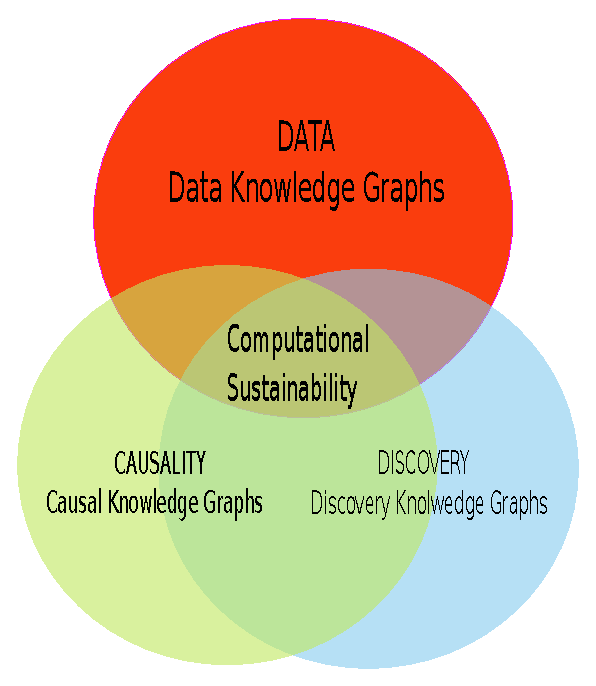
\includegraphics[width = 0.5\textwidth]{Fig0.pdf}\\
	 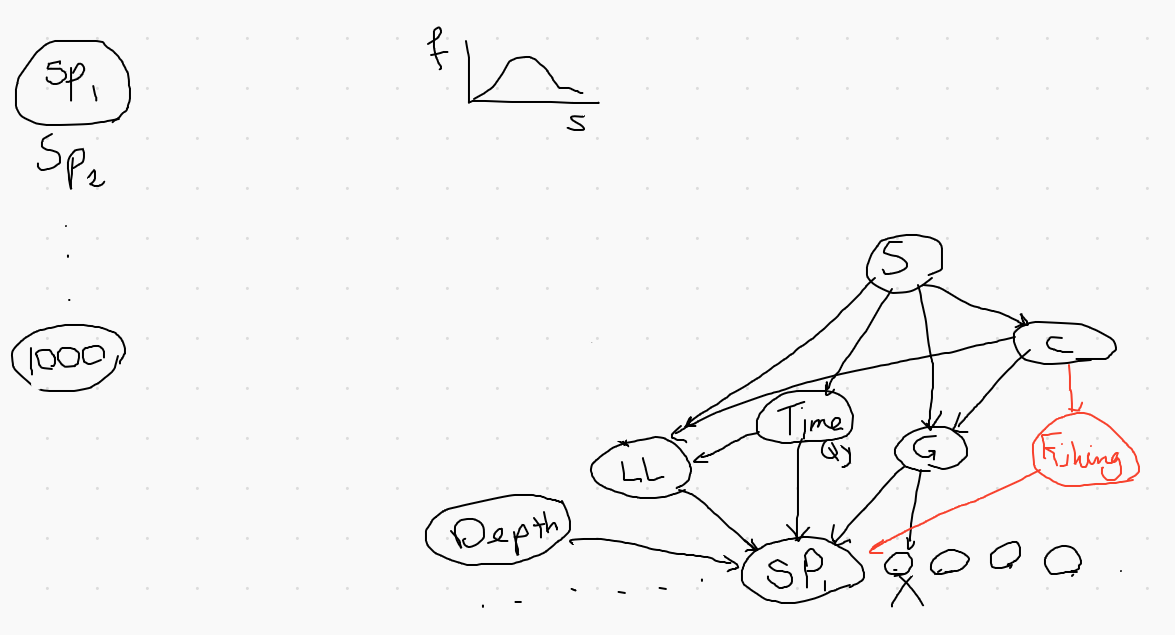
\includegraphics[width = 1\textwidth]{Fig1BN.png}
	 \caption{Computational sustainability is at the intersection of data, causality and discovery knowledge graphs. Data knowledge graphs introduce data fusion and semantics to disparate databases. Causality knowledge graphs make inferences about the processes explaining the empirical patterns observed in the data knowledge graphs. Discovery knowledge graphs find novel paths not observed in the empirical patterns but of relevance to increase sustainability.}
\end{figure}   

\begin{figure}[H]
	 \centering
	 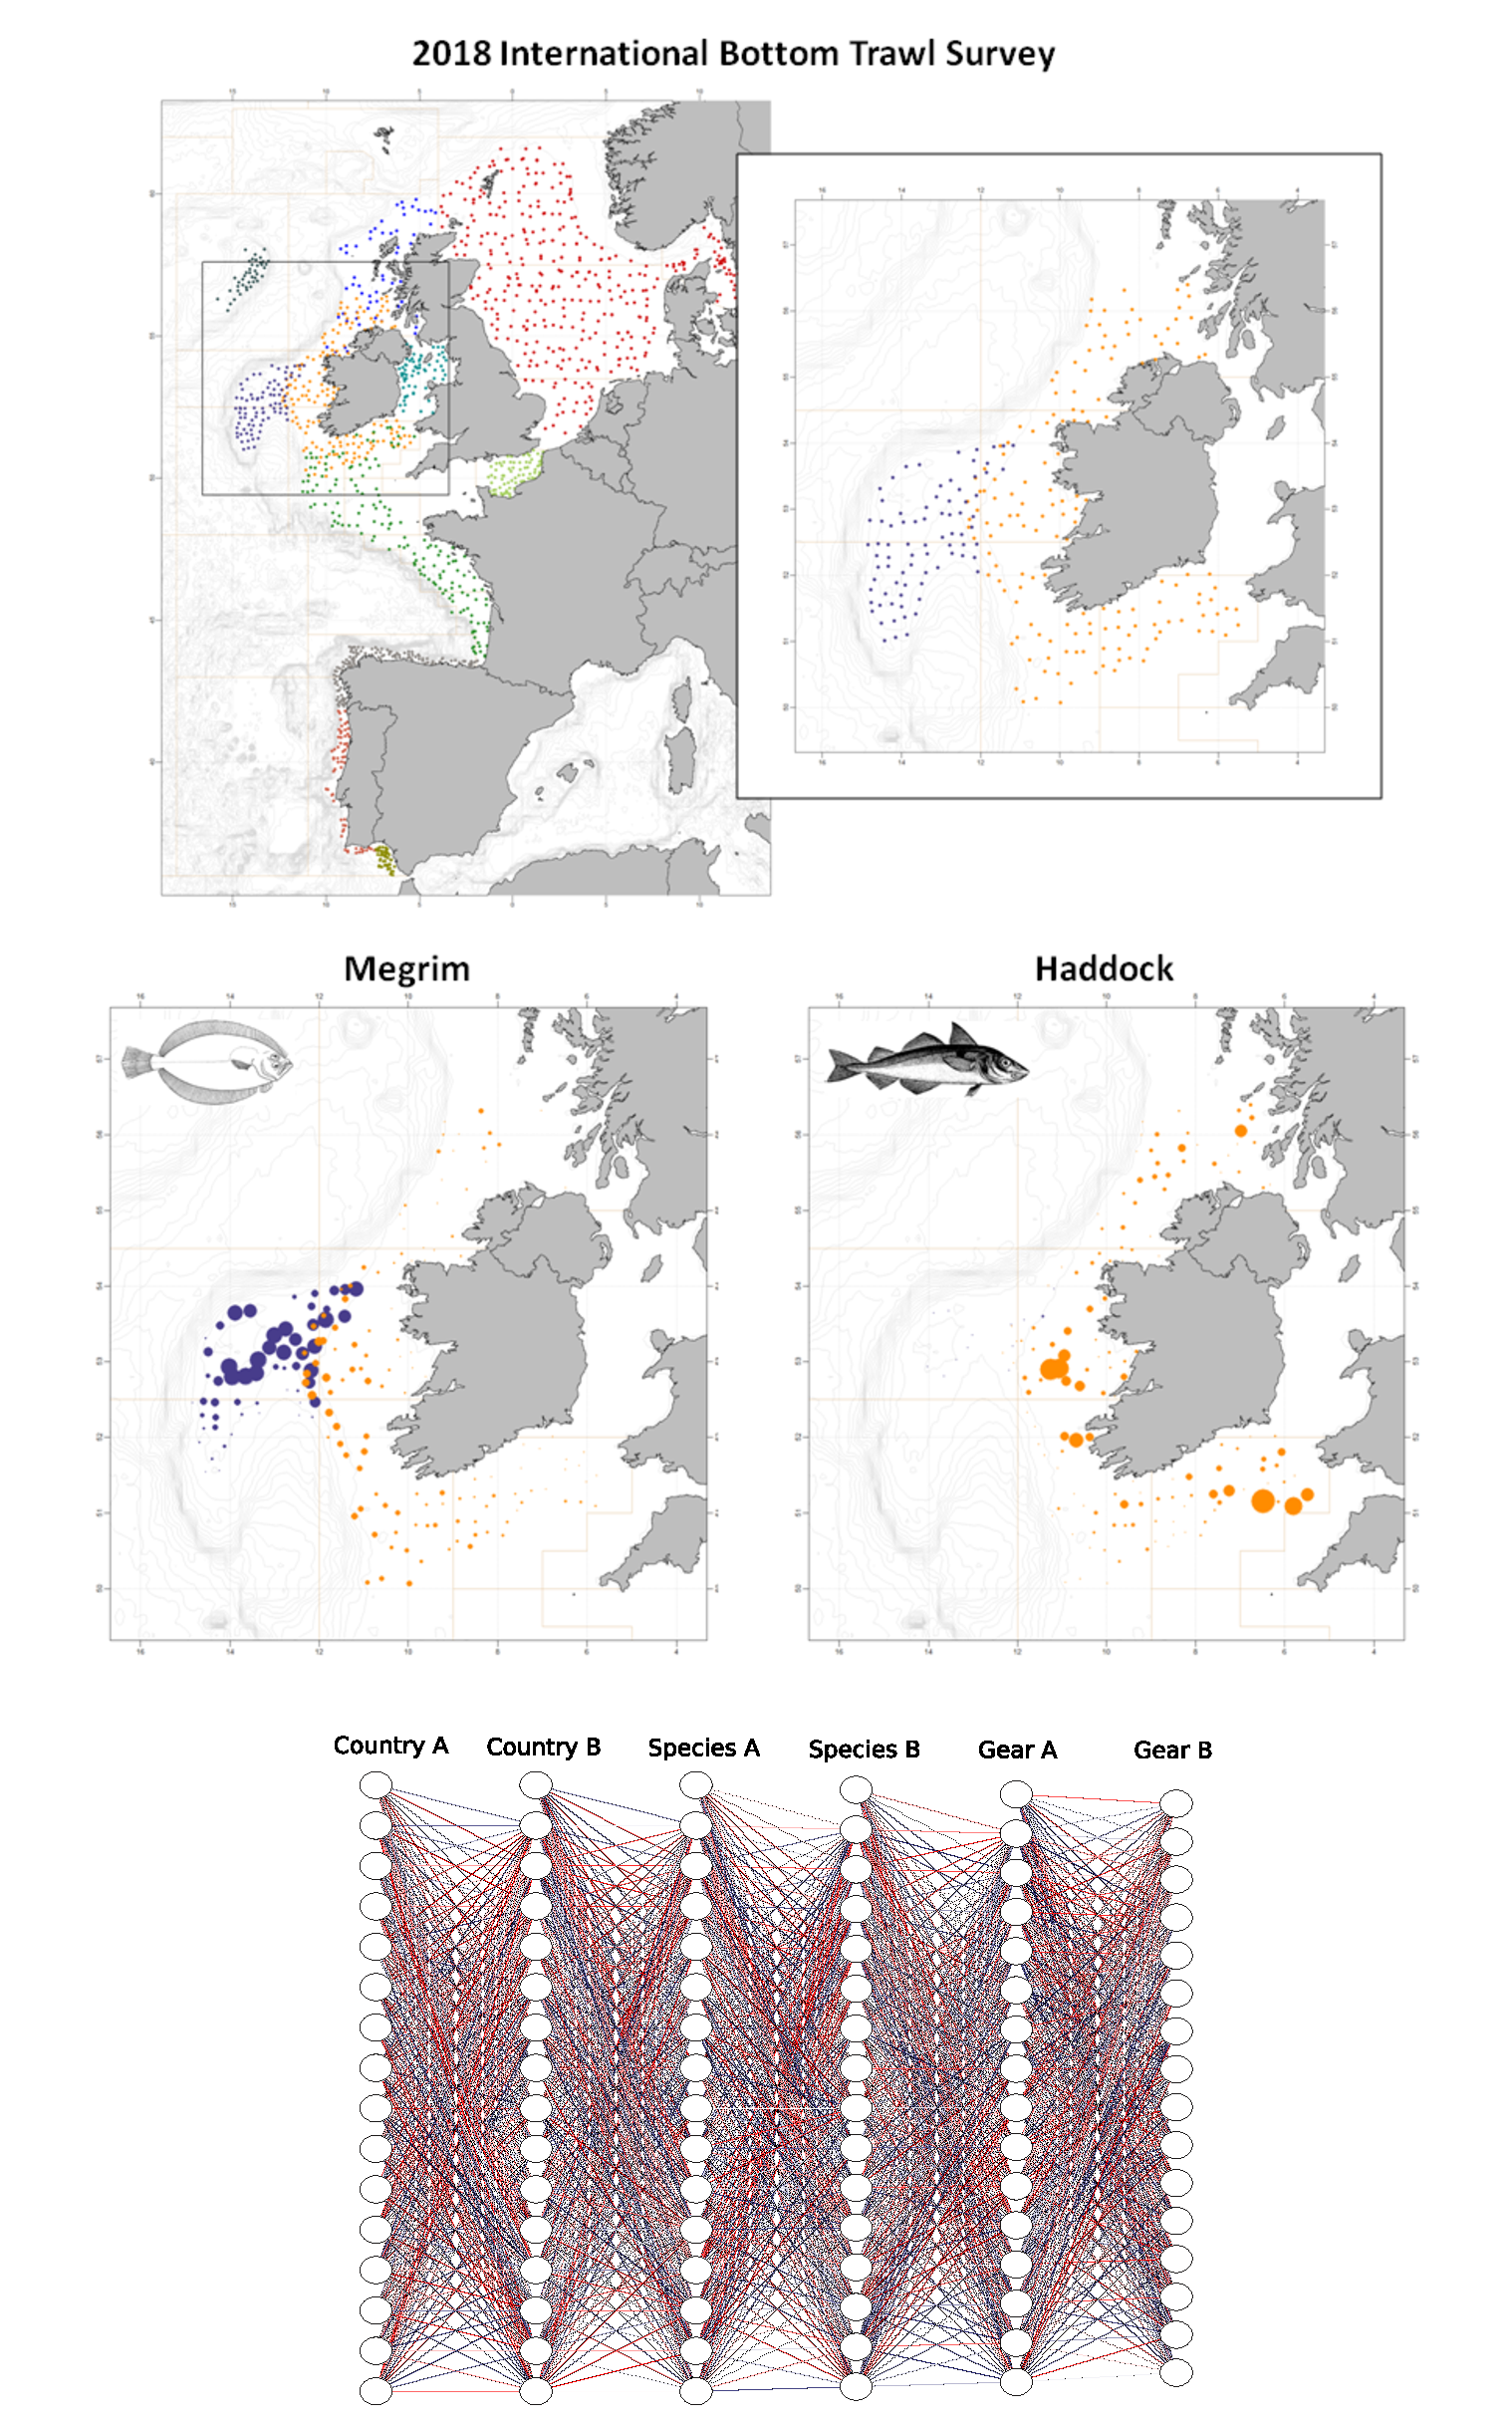
\includegraphics[width = 0.75\textwidth]{casestudy.pdf}
	 \caption{Computational sustainability applied to the sustainability of the Ocean case study combining many species, human groups and technologies. Top left) Zoomed in is the Irish Ground Fish Survey (IE-IGFS, Orange) and the Spanish Survey on the Porcupine Bank (PORC, Blue). Countries produce strong bias in the distributions maps because they use different Gears according to their commercial interest (Compare Megrim vs. Haddock samplings). Bottom) Each country, species and technology is composed of many nodes: a country contains fishery, environmental agencies, stakeholders, etc. A species contains size-classes, habitat preference, species interactions, etc. Red and blue links mean competition and cooperation links connecting each pair of nodes.}
\end{figure}

\begin{figure}[H]
	 \centering
	 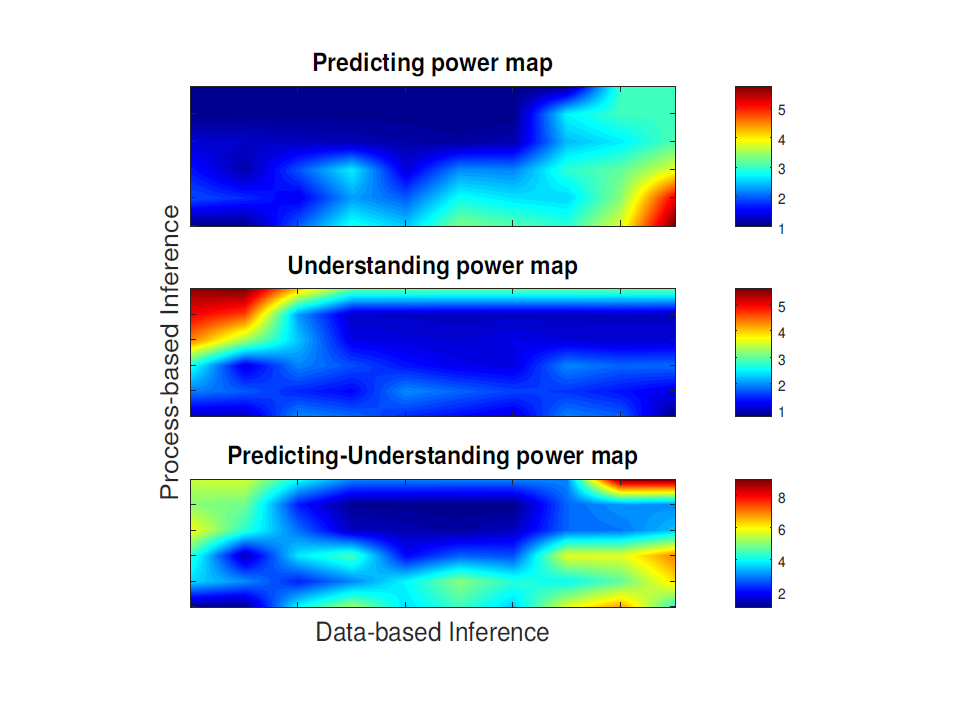
\includegraphics[width = 1\textwidth]{Fig1.png}
	 \\
	 \caption{CAPTION TO BE INCLUDED}
      \end{figure}

\begin{figure}[H]
	\centering
	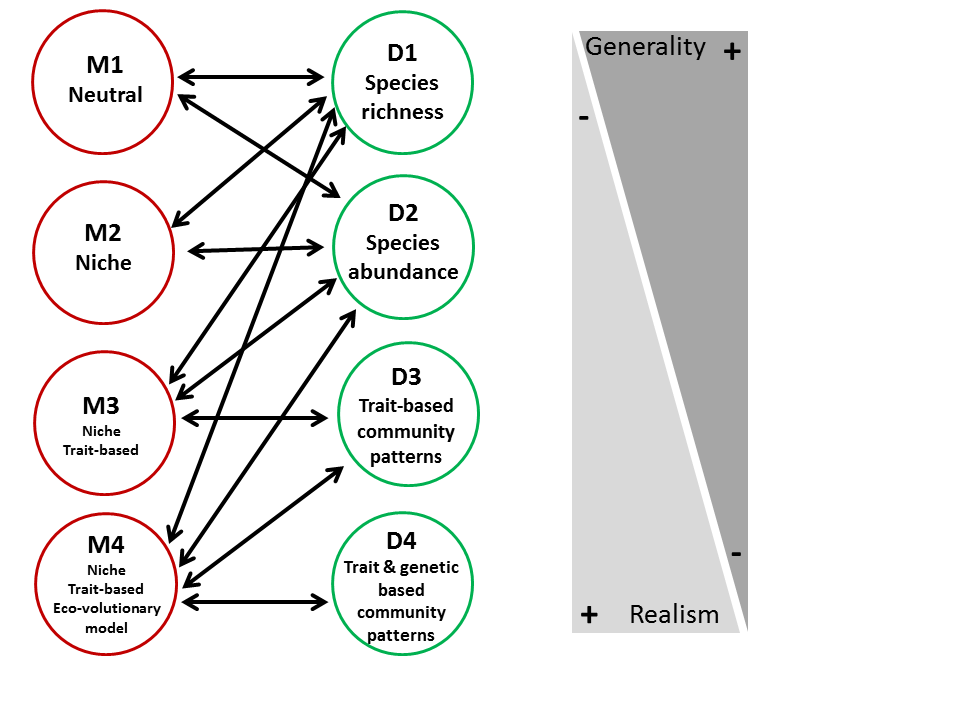
\includegraphics[width = 1\textwidth]{Fig2.png}
	\caption{Integration between models (M1-M4) and datasets (D1-D4). As model complexity increases (i.e., Realism) models produce more testable outputs but generality and tractability might decrease.}
\end{figure}

\newpage

\section{Box}

\vspace{0.25 in}
{\small \begin{tcolorbox}[colback=green!5!white,colframe=green!75!black]
  \textbf{Box 1: Open challenges in computational sustainability}. \\Connecting data, causal and discovery knowledge using eco-evolutionary diversification algorithms to understand the sustainability of the ecosystems is full of challenges. Here, we propose a framework to inspire data-causal-discovery synthesis in computational sustainability. The following five items are rooted in the fact that ecosystem patterns greatly vary in time and space and that most data is scattered within and among fields. With this in mind, what are the open challenges to connect the fundamentals of data-causal-discovery-based science to ecosystem sustainability?
\begin{itemize}
\item {\bf Time-dependent patterns and processes}: Ecosystem dynamics and therefore ecosystem sustainability greatly vary in space and time. At deep time, ecosystems change in size, number of species, functions, resilience, and more. Yet, the understanding of ecosystem sustainability in deep time is lacking. How does ecosystem sustainability change in space and time? Mention here the connection to macroecology, macroevolution, geodynamics and plate tectonics. Is there a model system to refer to? For example, how did the geodynamics (i.e., the topography of the ocean floor), and sea-level fluctuations alter ecosystem processes in our model system?
\item {\bf Spatiotemporal resolution and heterogeneity of data}: Data come with different resolution and heterogeneity levels within and between fields. Mention here the existing methods to standardize the data and also the existing gaps. How do we rarefy data within and between fields?
\item {\bf Dimensionality}: The availability of data to infer the number of factors driving the observed patterns is usually missing. The problem increases when connecting data from different fields. How can we infer robustly the dimensionality of an ecosystem? And how does dimensionality affect sustainability?    
\item {\bf Eco-evolutionary feedbacks}: There are many theoretical and empirical studies showing that changes in the ecological biotic or abiotic factors alter the frequency of phenotypes within populations from small to large organisms. Such fluctuating frequencies of phenotypes are, in some cases, rapidly evolving, and changing the ecological conditions of the ecosystem. This creates a loop between the ecology and the evolution within species, and this might be happening for many species in an ecosystem. How do feedbacks alter the sustainability of an ecosystem? 
\item {\bf Interaction networks}: Many studies have shown the topology of the factors governing the dynamics of species and communities and the structure of the interactions within and between species determine the stability properties of the ecosystem and its capacity to recover or to sustain continuous disturbances
\end{itemize}

We should connect these five points in a coherent framework -- Box 2 is a preliminary draft to do it.
\end{tcolorbox}}


{\small \begin{tcolorbox}[colback=green!5!white,colframe=green!75!black]
  \textbf{Box 2: Eco-evolutionary diversification algorithms in computational sustainability}\\
We validate our framework in Box 1 with a case study focusing on the sustainability of the ocean in federated networks, where many heterogeneous groups of species, humans, and technologies coexist exploiting resources in complex ecosystems.  Also, we aim to connect novel computational sustainability approaches to fully reproducible open-source software solutions of a science-enabled technology to connect knowledge-inspired societies to global sustainability challenges. In our model system, international programs for exploration of the oceans involve many countries collecting biodiversity data using different protocols and technologies (\cite{ices}). The data is then used to understand the spatiotemporal dynamics of the ecological communities as a baseline to inform the status of the ecosystems and fisheries. Each country collects data with different technology, i.e., gear systems, mostly driven by its commercial interests in specific species. This results in countries collecting heterogeneous and biased data about the same species, making it difficult to obtain accurate distribution maps of species (Figure 2). 

This is a tragedy of commons situation \cite{Hardin1968,Ostrom1990,Ecoffet2020} in the context of evolving ecosystems \cite{Rankinetal2007}: Many heterogeneous nodes (i.e., countries with different interests, groups, funding and conservation strategies, etc) exploit resources (i.e., species within ecosystems composed by a network of interacting species) using different technologies (i.e., gear systems and others technologies). Many of these ecosystems are overexploited. And yet, science-based technologies, providing forecasting scenarios and accounting for biased biodiversity data (i.e., species and environment), technologies (i.e., gear systems and other), and human groups with different interest within and between countries, to mitigate risks and enhance global cooperation scenarios in such multidimensional ecosystems are not in place. 

How do we account for diversifying technologies, species and human behaviours? For example, a social group represents a set of actors with multiple traits. In this context, groups are represented with evolving environmental and technological traits. We can formally describe these features as a distribution-fishery cooperation-competition matrix,
  $\mathcal{C}^{2}$, as follows:
  \vspace{-0.20 in}\\
\begin{center}
  $\mathcal{C}^2$ = \bordermatrix{~ &
    $\mathcal{F}^{i}_{\mathcal{A}_{g},\mathcal{B}_{g}}(c)$ &
    $\mathcal{F}^{i}_{\mathcal{A}_{g},\mathcal{B}_{g}}(nc)$ \cr
    $\mathcal{D}^{i}_{\mathcal{A}_{g},\mathcal{B}_{g}}(c)$ &
    $c(\varphi)$ & $c(\Phi), nc(\gamma_{A_{g}},\gamma_{B_{g}})$ \cr
    $\mathcal{D}^{i}_{\mathcal{A}_{g},\mathcal{B}_{g}}(nc)$ &
    $nc(\Phi_{A_{g}},\Phi_{B_{g}}), c(\gamma)$ &
    $nc(\phi_{A_{g}},\phi_{B_{g}})$ \cr}, 
    \vspace{-0.05 in}
\end{center}
where $\mathcal{D}^{i}_{\mathcal{A}_{g},\mathcal{B}_{g}}$, $\mathcal{F}^{i}_{\mathcal{A}_{g},\mathcal{B}_{g}}$ represent respectively the distribution map and fishery of species $i$, group $g$ within countries $\mathcal{A}$ and $\mathcal{B}$, and $c$ and $nc$ refer to cooperation and non-cooperation, respectively. The evolutionary diversification-inspired functions represent environmental and technological traits with different degrees of complexity in the $\mathcal{C}^2$ matrix: If the two groups within or between the countries cooperate, $c(\varphi)$, then the environmental and technological rate change, $\varphi$, is synchronized between groups to evolve towards decreasing Gear bias and make distribution maps and the fishery sustainable. This can be called the neutral scenario. On the other side, if the two groups decide not to cooperate, $nc(\phi_{A_{g}},\phi_{B_{g}})$, then the environmental and technological rate changes are given by $\phi_{A_{g}}$ and
$\phi_{B_{g}}$ respectively with each group following changes of their own gears, i.e., the GOV for the Ireland group and the Baka Gear for Spain group,
independently of the other and as a function of their fishery interest. There is no interest in decreasing bias in species distribution maps making fishery potentially non-sustainable in this case. In the last two scenarios groups enter in cooperation for the distribution
map of species $i$, but not in the fishery ($c(\Phi), nc(\gamma_{A_{g}},\gamma_{B_{g}})$), or they do cooperate in the fishery for species $i$ but not for the distribution map of species $i$ ($nc(\Phi_{A_{g}},\Phi_{B_{g}}), c(\gamma)$). The situation for cooperation in the distribution maps follows agreements between the two groups to technological changes in the Gear but still preserving their GOV and the Baka Gears for fisheries. Our approach explores classes of evolving functions within the cooperation-competition matrix combining them to automated Bayesian graphs ensuring the search, the evaluation of models, trading-off complexity, fitting to the data and quantify resource usage and recovery \citep{Guimera2020,Steinruecken}.
\end{tcolorbox}}


\newpage
\bibliographystyle{evolution}
\bibliography{Biblio_deepbios}

\end{document}
